\section{Introdução à linguagem c}

\begin{frame}{Meu primeiro programa}
    \fontsize{12pt}{15.2}\selectfont{
	Estrutura básica de um programa em C. 
	
	Code::Blocks IDE \url{www.codeblocks.org}
		
	\vspace{0.5em}
	\centering
    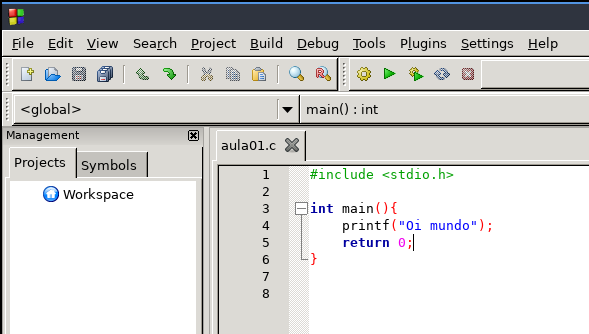
\includegraphics[width=0.75\textwidth]{images/fig-aula01-oi-mundo.png}

    }\par

	\vspace{1em}
\end{frame}

\begin{frame}[fragile]{Programa 001}

\lstinputlisting[style=CBruno,caption=Exemplo de Código]{codigos/c/001-oimundo.c}

\end{frame}

\begin{frame}{Meu primeiro programa}
    \fontsize{12pt}{15.2}\selectfont{
	Estrutura básica de um programa em C.
		
	\vspace{1em}
	\centering
    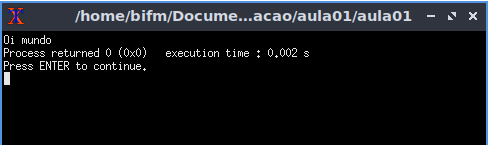
\includegraphics[width=0.8\textwidth]{images/fig-aula01-oi-mundo-p2.png}

    }\par

	\vspace{1em}
\end{frame}


\begin{frame}{Comentário}
    \fontsize{12pt}{15.2}\selectfont{
	São blocos de códigos ignorados pelo compilador.
		
	\vspace{1em}
	// comentário de linha
	
	/*
	
	comentário de bloco
	
	*/
	
    }\par

	\vspace{1em}
\end{frame}



\begin{frame}{Identação}
    \fontsize{14pt}{15.2}\selectfont{
	Identar um código nada mais é que separar os códigos em blocos através de tabulação.
		
	\vspace{1em}
	Não identado:
	
	\#include <stdio.h>int main()\{printf(``Oi mundo'');return 0;\}
	

    }\par
    
    \vspace{1em}
    
    *O código acima não está identado. Note como está complicado de ler, apesar de ser um código extremamente simples.
    
	\vspace{1em}
\end{frame}

\begin{frame}{Tipos de Dados}
    \fontsize{14pt}{15.2}\selectfont{
    
	A linguagem C possuí 5 (cinco) tipos básicos de dados: \textbf{char}, \textbf{int}, \textbf{float}, \textbf{void} e \textbf{double}.
	
	\vspace{1em}
	
	O \textbf{void} é um tipo de dado vazio (sem valor).
	
	\vspace{1em}
	
	Para cada tipo de dado existem modificadores de tipo, estes são 4 (quatro): \textbf{signed}, \textbf{unsigned}, \textbf{long} e \textbf{short}.
	
	\vspace{1em}
	
	Para o \textbf{float} nenhum modificado pode ser aplicado; assim como para o \textbf{double} podemos aplicar APENAS o \textbf{long}.
		
    }\par
    
    \vspace{1em}

\end{frame}


\begin{frame}{Tipos de Dados}
    \fontsize{14pt}{15.2}\selectfont{
    
	\begin{tabular}{|l|l|l|}
	\hline
Nome & Característica  & Intervalo \\ \hline
\textbf{char} & carácter/literal  &  -128 a 127  \\ \hline
\textbf{int} & número inteiro & -32.768 a 32.767  \\ \hline
\textbf{float} & ponto flutuante em simples precisão  & 3.4 E-38 a 3.4E+38 \\ \hline
\textbf{double} & ponto flutuante em dupla precisão  & 1.7 E-308 a 1.7E+308  \\ \hline
\textbf{void} & vazio & (sem valor)   \\ \hline

\end{tabular}
		
    }\par
    
    \vspace{1em}

\end{frame}


\begin{frame}{Tipos de Dados}
    \fontsize{14pt}{15.2}\selectfont{
    Qualificadores de tipo \textbf{unsigned} e \textbf{signed} podem ser aplicados a tipos \textbf{char} e \textbf{int}:
    
    \vspace{5mm}
    
    \textbf{unsigned} - considera apenas valores positivos.
    
    \vspace{5mm}
    
    
    \textbf{signed} - consideram valores positivos e negativos. por padrão todos são signed.
		
    }\par
    
    \vspace{1em}

\end{frame}

\begin{frame}{Tipos de Dados}
    \fontsize{14pt}{15.2}\selectfont{
    Qualificadores de tipo \textbf{long} e \textbf{shot} podem ser aplicados a tipos \textbf{int} e \textbf{double}. Entretanto, para \textbf{double}, apenas o \textbf{long} é aplicado.
    
    \vspace{5mm}
    
    \textbf{short} - aplicável apenas para \textbf{int}. Reduz pela metade o tamanho.
    
    \vspace{5mm}
    
    
    \textbf{long} - aplicável para \textbf{int} e \textbf{double}.
		
    }\par
    
    \vspace{1em}

\end{frame}



\begin{frame}{Tipos de dados}
	\vspace{1em}


\begin{tabular}{|l|r|c|r|r|}
\hline
\multirow{2}{*}{Tipo} & Número & 
Formato  & \multicolumn{2}{c|}{Intervalo}\\ 

& de bytes & Sintaxe printf & 
Início & Fim \\ \hline 

char& 1& \%c & -128 & 127 \\ \hline
unsigned char & 1& \%c & 0& 255 \\ \hline
signed char & 1& \%c & -128 & 127 \\ \hline
int & 4 & \%d & -32.768& 32.767\\ \hline
unsigned int& 4 & \%u & 0& 65.535\\ \hline
signed int& 2 & \%i & -32.768& 32.767\\ \hline
short int & 2 & \%hi& -32.768& 32.767\\ \hline
unsigned short int& 2 & \%hu& 0& 65.535\\ \hline
signed short int& 2 & \%hi& -32.768& 32.767\\ \hline
long int& 8 & \%li& -2.147.483.648 & 2.147.483.647 \\ \hline
signed long int & 8 & \%li& -2.147.483.648 & 2.147.483.647 \\ \hline
unsigned long int & 8 & \%lu& 0& 4.294.967.295 \\ \hline
double & 8 & \%d& - & - \\ \hline
long double & 16 & \%d& - & - \\ \hline
float & 4 & \%f & - & - \\ \hline
long (inteiro) & 4 & \%f & - & - \\ \hline
short (inteiro) & 2 & \%f & - & - \\ \hline
\end{tabular}

	
% 	\centering
%     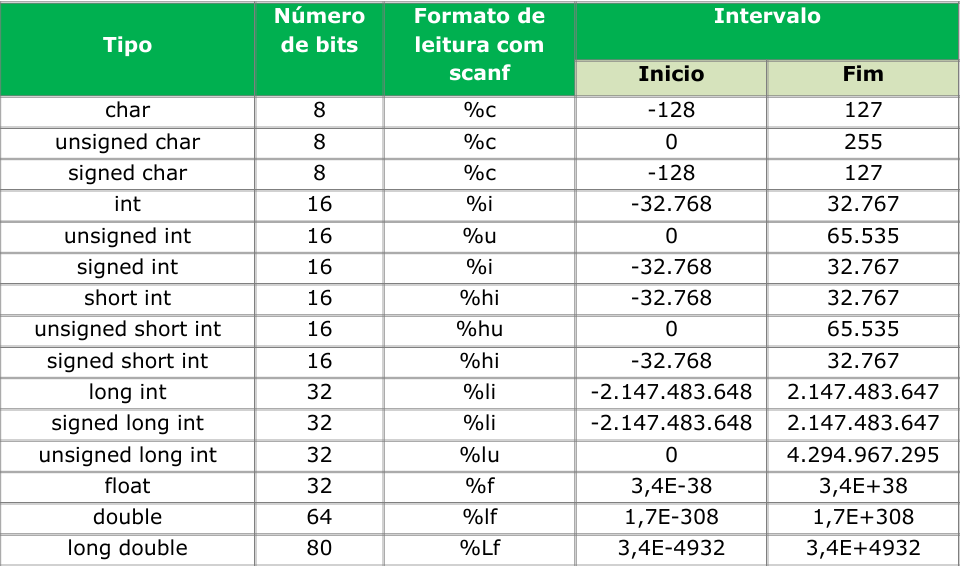
\includegraphics[width=0.85\textwidth]{images/fig-tipo-de-dados.png}
\end{frame}


\begin{frame}{Tipos de Dados}
    \fontsize{14pt}{15.2}\selectfont{
    \textbf{Declaração de variável}: 
    \vspace{1em}
    }\par
    \fontsize{12pt}{15.2}\selectfont{
        tipo\_da\_variavel nome\_da\_variavel = valor\_inicial\_da\_variavel; 
	}
    
    \vspace{1em}

    \fontsize{14pt}{15.2}\selectfont{
    \textbf{Declaração de variáveis de um mesmo tipo}: 
    \vspace{1em}
    }\par
    \fontsize{12pt}{15.2}\selectfont{
        tipo\_da\_variavel nome\_da\_variavel1 = valor1, nome\_var2 = valor2; 
	}

	\vspace{1em}
\end{frame}

\begin{frame}{Boas práticas}
    \fontsize{16pt}{15.2}\selectfont{
    Ao nomear uma variável seja objetivo, use nomes fáceis de entender e se necessário faça um comentário acima da variável explicando sua utilidade. Em nomes compostos separe-os utilizando underline.
    \vspace{1em}
    }
\vspace{1em}

\end{frame}


\begin{frame}{Constantes de barra invertida}

\begin{tabular}{|c|l|}
\hline
\textbf{Constante}                        & \textbf{Representação}   \\ \hline
\textbackslash{}n                & Nova Linha      \\ \hline
\textbackslash{}t                & Tab Horizontal  \\ \hline
\textbackslash{}v                & Tab Vertical    \\ \hline
\textbackslash{}"                & Aspas Duplas    \\ \hline
\textbackslash{}'                & Aspas Simples   \\ \hline
\textbackslash{}\textbackslash{} & Barra Invertida \\ \hline
\textbackslash{}a                & Sinal sonoro/Beep     \\ \hline

\end{tabular}


	\vspace{1em}
\end{frame}


\begin{frame}{Operadores aritméticos e de atribuição}

\begin{tabular}{|c|l|}
\hline
\textbf{Operador} & \textbf{Ação}   \\ \hline
+ & Soma      \\ \hline
- & Substração  \\ \hline
* & Multiplicação    \\ \hline
/ & Divisão     \\ \hline
\%  & Resto da divisão   \\ \hline
++ & Incremento\\ \hline
-- & Decremento     \\ \hline

\end{tabular}


	\vspace{1em}
\end{frame}



\begin{frame}{Operadores de Racionais/lógicos}


\begin{tabular}{|c|l|}
\hline
\textbf{Operador} & \textbf{Ação}   \\ \hline
> & Maior do que      \\ \hline
>= & Maior ou igual a  \\ \hline
< & Menor do que    \\ \hline
<= & Menor ou igual a     \\ \hline
==  & Igual a   \\ \hline
!= & Diferente de\\ \hline
\&\& & AND (E) \\ \hline
|| & OR (OU) \\ \hline
! & NOT (NÃO) \\ \hline

\end{tabular}

	\vspace{1em}
\end{frame}

\begin{frame}{Tabela verdade}
    \fontsize{12pt}{15.2}\selectfont{
	\vspace{1em}
	\centering
    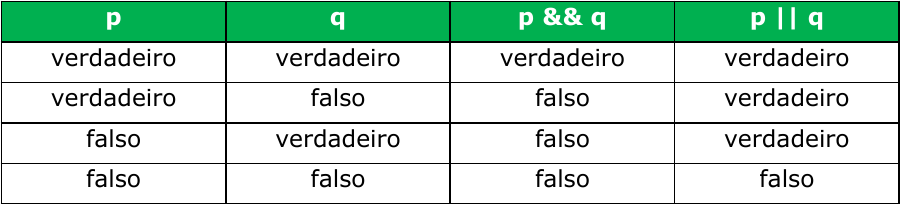
\includegraphics[width=0.8\textwidth]{images/fig-tabela-verdade.png}

    }\par

	\vspace{1em}
\end{frame}


\begin{frame}{Tabela de Precedência}
    \fontsize{12pt}{15.2}\selectfont{
	\vspace{1em}
	\centering
    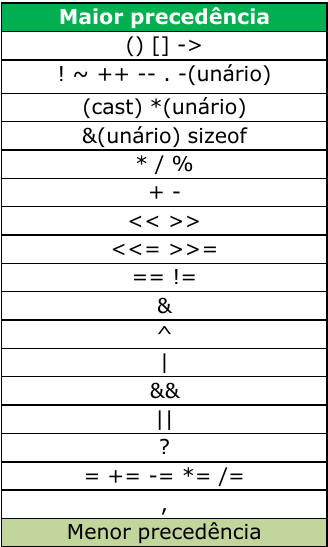
\includegraphics[width=0.35\textwidth]{images/fig-tabela-precedencia.png}

    }\par

	\vspace{1em}
\end{frame}



\begin{frame}{Resolução L3Q7}
    \fontsize{12pt}{15.2}\selectfont{
	Resolução da questão 7 (Q7), lista 3 (L3).
		
	\vspace{0.5em}
	\centering
    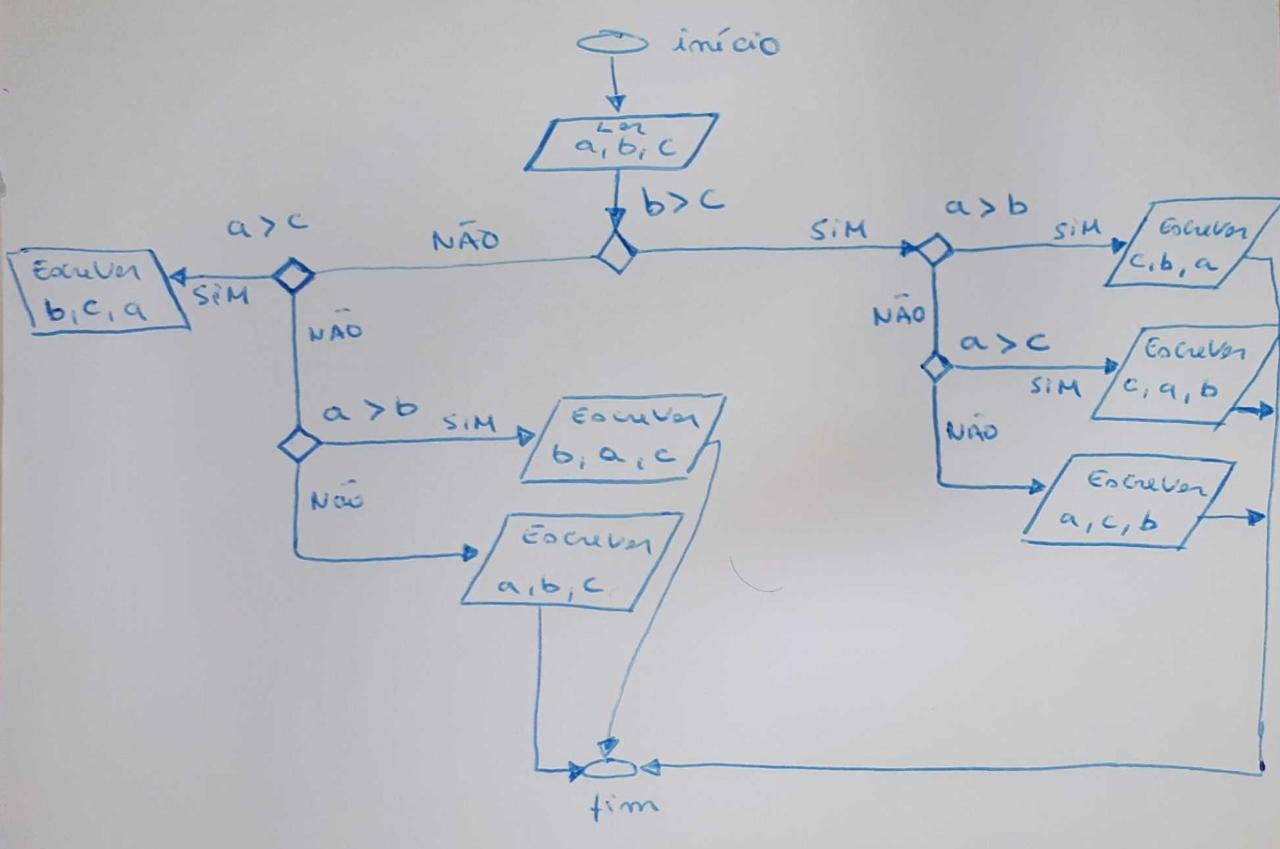
\includegraphics[width=0.7\textwidth]{images/fig-l3-q7.jpeg}

    }\par

	\vspace{1em}
\end{frame}


\begin{frame}{Entrada e saída de dados}
    \fontsize{14pt}{15.2}\selectfont{
    
    \vspace{5mm}
    
    \textbf{scanf(), gets(), fgets()} - utilizados para entrada de dados.
    
    \vspace{5mm}
    
    
    \textbf{printf()} - utilizado para saída de dados.
		
    }\par
    
    \vspace{1em}

\end{frame}



\begin{frame}{Entrada e saída de dados}

\begin{tabular}{|c|l|}
\hline
\textbf{Código} & \textbf{Formado}   \\ \hline
\%c & Receber um caractere      \\ \hline
\%d & Receber número inteiro  \\ \hline
\%f & Receber número de ponto flutuante   \\ \hline
\%s & Receber uma cadeira de caracteres    \\ \hline

\end{tabular}


\end{frame}


\begin{frame}{Entrada e saída de dados}
    \fontsize{13pt}{14}\selectfont{
    
    \vspace{5mm}
    
    \textbf{scanf()} - a entrada é finalizada assim que um espaço em branco (whitespace) é encontrado. É possível burlar usando scanf(``\%[$\text{\^{}}$$\textbackslash$n]s'', x) % , newline ou EOF.
    
    \vspace{5mm}
    
    \textbf{gets()} - considera um espaço em branco como parte da cadeia de entrada e termina a entrada ao encontrar newline ou EOF.
    
    \vspace{5mm}
    
    % \textbf{fgets()} - mais confiável que os outros dois, ele evita erros de estouro de buffer, minimizando riscos de segurança. Porém, insere uma quebra de linha ao final.
		
    }\par
    
    \vspace{1em}

\end{frame}


\begin{frame}[fragile]{Exemplo 002}

\lstinputlisting[style=CBruno,caption=Exemplo de Código]{codigos/c/002-scanf.c}

\end{frame}

\begin{frame}[fragile]{Exemplo 003}

\lstinputlisting[style=CBruno,caption=Exemplo de Código]{codigos/c/003-gets.c}

\end{frame}

% \begin{frame}[fragile]{Entrada e saída de dados}

% \lstinputlisting[style=CBruno,caption=Exemplo de Código]{codigos/c/004-fgets.c}

% \end{frame}



\begin{frame}{Estruturas de Controle de Fluxo}
    \fontsize{14pt}{14}\selectfont{
    
        \begin{itemize}
            \item São responsáveis por controlar o fluxo do programa 
            \item Testam condições. 
            \item Algumas são conhecidas como ``loops''.
        \end{itemize}
    }\par
    \vspace{1em}
\end{frame}




\begin{frame}{if-else}
    \fontsize{14pt}{14}\selectfont{
    A estrutura \textbf{if-else} é utilizada para tomada de decisões, quando uma condição é válida ou não.
         \vspace{1em}
        
        if ( condicao ) \{ 
        
        \hspace{5mm}    bloco\_de\_comando 
            
        \} else \{ 
        
        \hspace{5mm}    bloco\_de\_comando 
            
        \}
        
    }\par
    \vspace{1em}
\end{frame}

\begin{frame}[fragile]{Exemplo 004}

\lstinputlisting[style=CBruno,caption=Exemplo de Código]{codigos/c/004-if-else.c}

\end{frame}




\begin{frame}{switch}
    \fontsize{13pt}{14}\selectfont{
    O \textbf{switch} também é utilizado para tomada de decisões, porém cria um código mais limpo. Com ele você pode testar uma variável em relação a diversos valores pré- estabelecidos.
    
         \vspace{1em}
        
        switch ( variável ) \{ 
        
        \hspace{5mm}   case 1:
        
        \hspace{5mm}\hspace{5mm}    bloco\_de\_comando 
        
        \hspace{5mm} \hspace{5mm} break;
        
        \hspace{5mm} default: 
        
        \hspace{5mm}\hspace{5mm}    bloco\_de\_comando 
            
        \}
        
    }\par

\end{frame}


\begin{frame}[fragile]{Exemplo 005}

\lstinputlisting[style=CBruno,caption=Exemplo de Código]{codigos/c/005-switch.c}

\end{frame}


\begin{frame}{switch}
    \fontsize{14pt}{14}\selectfont{
    *obs: trabalha com números inteiros.
        
    }\par
    \vspace{1em}
\end{frame}

\begin{frame}{while}
    \fontsize{14pt}{14}\selectfont{
    O \textbf{while} é uma estrutura de repetição, utilizada para criar os chamados ``loops'' de um programa. O código dentro do bloco repetirá enquanto a condição não for verdadeira.
    
         \vspace{1em}
        
        while ( condicao ) \{ 

        \hspace{5mm}   bloco\_de\_comando 
            
        \}
        
    }\par
      \vspace{1em}
      
    *É utilizando quando não sabe-se a quantidade de repetições.
  
\end{frame}

\begin{frame}[fragile]{Exemplo 006}

\lstinputlisting[style=CBruno,caption=Exemplo de Código]{codigos/c/006-while.c}

\end{frame}



\begin{frame}[fragile]{for}
    \fontsize{14pt}{14}\selectfont{
   Assim como o \textbf{while} o \textbf{for} é utilizado para criar estruturas de repetição.
    
         \vspace{1em}
        
        for ( inicializacao; condicao; incremento ) \{ 

        \hspace{5mm}   bloco\_de\_comando 
            
        \}
        
    }\par
    
    %Document body
\begin{lstlisting}[style=CBruno]
for(i=0; i < 10; i++){
    //bloco de comando
}
\end{lstlisting}

    \vspace{1em}
\end{frame}

\begin{frame}[fragile]{Exemplo 007}

\lstinputlisting[style=CBruno,caption=Exemplo de Código]{codigos/c/007-for.c}

\end{frame}

